\documentclass{article}
\usepackage[utf8]{inputenc}
\usepackage{graphicx}
\graphicspath{ {./imgs/} }
\usepackage{geometry}
\usepackage{indentfirst}
\usepackage[spanish]{babel}
\usepackage{amsmath}
\usepackage{amssymb}
\usepackage{hyperref}
\usepackage{graphicx}
\usepackage[nottoc]{tocbibind}
\usepackage{tcolorbox}
\usepackage{listings}
\usepackage{color}
\usepackage{float}
\usepackage{minted}
\newminted{python}{}
\usepackage{verbatim}
\hypersetup{
    colorlinks=true,
    linkcolor=blue,
    filecolor=magenta,      
    urlcolor=cyan,
}

\geometry{
 a4paper,
 left=23mm,
 right=23mm,
 top=32mm,
 }
\definecolor{mygreen}{RGB}{28,172,0} 
\definecolor{mylilas}{RGB}{170,55,241}
\lstset{language=Python,
    breaklines=true,%
    keywordstyle=\color{blue},%
    morekeywords=[2]{1}, keywordstyle=[2]{\color{black}},
    identifierstyle=\color{black},%
    stringstyle=\color{mylilas},
    commentstyle=\color{mygreen},%
    showstringspaces=false,%without this there will be a symbol in the places where there is a space
    numbers=left,%
    numberstyle={\small \color{darkgray}},% size of the numbers
    numbersep=0pt, % this defines how far the numbers are from the text
    emph=[1]{for,end,break},emphstyle=[1]\color{red}, %some words to emphasise
    tabsize=4
}

\begin{document}
\pagenumbering{gobble}
%-----------------------------------PORTADA------------------------------------
\vspace{2cm}
\begin{center}
    
\includegraphics[scale=1.6]{logo-unam-bw.jpg}
    \hspace{6cm}
    
\includegraphics[scale=0.29]{imgs/logo-iimas.png}
\end{center}
\vspace{1cm}
\begin{center}
    \textbf{{\Huge Proyecto Final}} 
    \\ \vspace{0.5cm}
    \huge Algoritmos de Computaci\'on Evolutiva
    \\ \vspace{0.5cm}
    \textit{\Large Computaci\'on Concurrente }
    \\ \vspace{0.5cm}
    \Large I.I.M.A.S.
    \\ \vspace{0.2cm}
    \Large U.N.A.M
    \\ \vspace{1cm}
    \huge Barajas Cervantes Alfonso\\
    \huge Cabello Figueroa Israel\\
    \huge Cerritos Lira Carlos  \\
    \huge Franco López Benito Vicente
    \\ \vspace{1.2cm}
    \Large Dr. \'Oscar Alejandro Esquivel  Flores
    \\ \vspace{1cm}
    \Large 22 de enero del 2021
\end{center}
%-----------------------------------------CONTENIDO----------------------------------------
\newpage
\pagenumbering{arabic}
\section{Requerimientos}

\section{Organizacion}
#Investigar algoritmos evolutivos aunque sea para una solución de un problema sencillo
Propuesta para la primera Fase de los Rquerimientos:\\
1.-Seleccionar 5-10 ejemplos concretos que puedamos seguir \\
2.-Elegir alguno de ellos y entenderlo bien \\
3.-Trabajar sobre un colab y decidir que parte del programa podria empezar a desarrollar cada quien\\
4.-En paralelo ir llenando, la introducción y la explicación de nuestro problema\\
5.- Llenar las conclusiónes de nuestro proyecto\\



\section{Requerimientos}
\begin{enumerate}
    \item{Realizar la investigación correspondiente a los algoritmos evolutivos y su aplicación}
    \item{Evaluar,elegir y analizar un algoritmo de interes que pueda ser ejecutado de manera concurrente}
    \item{Considerar un problema de aplicación del algoritmo evolutivo elegido en el punto anterión}
    \item{Plantear el problema y hacer el analisis de la implementación concurrente}
    \item{Elaborar el análisis correspondiente de la implementación considerando
    \begin{itemize}
        \item Validación de resultados
        \item Tiempo de ejecución de la implementación secuencial
        \item Tiempo de implementación de la ejecución concurrente
    \end{itemize}}
   
\end{enumerate}


\section{Introducción}

\subsection*{Marco Hist\'orico}

En 1859, Darwin publica su libro El origen de las especies que levantó agrias
polémica en el mundo científico por las revolucionarias teorías que sostenían que las
especies evolucionan acorde al medio, para adaptarse a éste.
De esta manera el universo pasaba de ser una creación de Dios estática y perfecta y
se planteaba como un conjunto de individuos en constante competición y evolución para
poder perpetuar su especie en el tiempo. Las especies se crean, evolucionan y
desaparecen si no se adaptan de forma que solo los mejores, los más aptos, los que
mejor se adapten al medio sobreviven para perpetuar sus aptitudes. 
De acuerdo con esta visión de la evolución, la computación ve en dicho marco un
claro proceso de optimización: se toman los individuos mejores adaptados –mejores
soluciones temporales –, se cruzan –mezclan–, generando nuevos individuos –nuevas
soluciones– que contendrán parte del código genético –información– de sus antecesores,
y el promedio de adaptación de toda la población se mejora.

La computación evolutiva se ha convertido en un concepto general adaptable para
resolución de problemas, en especial problemas difíciles de optimización, ella encuentra fuerza combinada con otras técnicas como lo es la computación concurrente. 

\subsection*{Algoritmos Evolutivos, Computaci\'on Evolutiva y m\'as}

La rama de la \text{computaci\'on evolutiva} es en si una rama que envuelve una gran comunidad de gente, ideas y de aplicaciones. Aunque sus raices genealogicas podemos tenerlos desde 1930, surgi\'o como la emergencia de una relativa tecnologia computacional digital no costosa en la d\'ecada de los 60, que sirvi\'o como un importante catalizador para la rama. La viabilidad de usar esta tecnolog\'ia fue de gran importancia para realizar simulaciones como herramiento para analizar sistemas mucho m\'as complejos que aquellos que se podr\'ian analizar matem\'aticamente.

Los algoritmos genéticos son herramientas que podemos usar aplicando aprendizaje máquina que algunas veces nos permite encontrar soluciones para problemas que podrían tener un número muy grande de potenciales soluciones. Cuando resolvemos un problema con un algoritmo genético en lugar de emplear una solución específica, necesitamos dar carácterísitcas y reglas a la solución para que estás sean aceptadas. Cuando estamos viendo por ejemplo si pensamos en la tarea de llenar un camión de carga, debemos establecer principios y reglas que restringan los posibles ordenes en que acomodemos las cosas, por ejemplo una primera regla podría ser meter las cosas más pesadas primero, las cosas frágiles al final, para colocarlas en sitios donde no se golpeen. Estás reglas restrigen el espacio de posibles soluciones.

\\
Ahora pensemos que estamos resolviendo un problema en particular de adivinar un numero, entre 1 y 1000, y tenemos solo diez opciones para adivinar. Si la única retroalimentación que tienes del número, es si escogiste correctamente, o incorrectamente, entonces tu mejor oportunidad es de 1 en 100 de adivinar el número. Con los algoritmos genéticos recibimos información adicional, dan una retroalimentación acerca de que tan cerca o lejos están de la solución.
Si en lugar de correcto o incorrecto recibimos este indicador, la probabilidad de encontrarlo es total, porque con búsqueda binaria podemos encontrar cualquier número entre 1 y 1000 en diez pasos.



\subsection{Clasificación de los algoritmos evolutivos}
\begin{enumerate}
    \item Estrategias Evolutivas:
Fue diseñada inicialmente
con la meta de resolver problemas de optimización discretos y continuos,
principalmente experimentales y considerados difíciles. Trabaja con vectores de
números reales Dcon desviaciones estándarD que codifican las posibles soluciones de
problemas numéricos. Utiliza recombinación o cruce (crossover aritmético), mutación y
la operación de selección, ya sea determinística o probabilística, elimina las peores
soluciones de la población y no genera copia de aquellos individuos con una aptitud por
debajo de la aptitud promedio.
  \item{Programación Evolutiva:}
  Inicialmente fue diseñada como un intento de crear inteligencia artificial.
La representación del problema se realiza mediante números reales (cualquier estructura
de datos), y emplea los mecanismos de mutación y selección. El procedimiento es muy
similar a las estrategias evolutivas con la diferencia de que no emplea la recombinación,
de tal forma que son denominadas en conjunto algoritmos evolutivos como una manera
de diferenciarlas de los algoritmos genéticos. 
\item{Algoritmos Genéticos:}
Modelan el proceso de evolución como una sucesión de
frecuentes cambios en los genes, con soluciones análogas a cromosomas. Trabajan con
una población de cadenas binarias para la representación del problema, y el espacio de
soluciones posibles es explorado aplicando transformaciones a éstas soluciones
candidatas tal y como se observa en los organismos vivientes: cruce, inversión y
mutación. Como método de selección emplean en mecanismo de la ruleta (a veces con
elitismo). Constituyen el paradigma más completo de la computación evolutiva ya que 
resumen de modo natural todas las ideas fundamentales de dicho enfoque. Son muy
flexibles ya que pueden adoptar con facilidad nuevas ideas, generales o específicas, que
surjan dentro del campo de la computación evolutiva. Además, se pueden hibridar
fácilmente con otros paradigmas y enfoques, aunque no tengan ninguna relación con la
computación evolutiva. Se trata del paradigma con mayor base teórica.
\end{enumerate}
\subsection{Procesos Evolutivos B\'asicos}
Un lugar bueno para empezar es preguntarse los componentes b\'asicos de un sistema evolutivo. La primer nota que debemos tomar en cuenta es que existen al menos dos posibles interpretaciones de un \textit{Sistema Evolutivo}. Es frecuentemente usado para describir un sistema que cambia con incrementos a lo largo del tiempo. La segunda interpretaci\'on es aquella que tiene un sentido biol\'ogico, es decir, que es un sistema evolutivo Darwiniano.

Para ello, precisamos saber lo que entendemos por un \textit{Sistema}. Una manera es identificando lo que precisamente constituye al sistema, es decir todas sus partes. A continuaci\'on se presenta el conseso de lo que se entiende por un sisteme evolucionario Darwiniano.
\begin{itemize}
    \item Una o m\'as poblaciones compiten por limitados recursos
    \item Noci\'on de que las poblaciones cambien din\'amicamente debido al nacimiento y la muerte de individuos.
    \item El concepto de la aptitud en donde refleja la habilidad de un individuo de sobrevivir y de reproducirse
    \item El concepto de  herencia variacional: la descendencia se parece mucho a sus padres, pero son no es identicos.
\end{itemize}
\subsection{Un primer ejemplo: Un simple Sistema Evolutivo}
La primera cuestión a afrontar es cómo representar a los individuos (organismos) que componen una población en evolución. Una técnica bastante general es describir a un individuo como un vector de longitud de las características L que se eligen presumiblemente debido a su relevancia (potencial) para estimar la aptitud de un individuo. Entonces, por ejemplo, los individuos podrían caracterizarse por:
\begin{equation*}
    < \textrm{color cabello, color ojos, color piel, altura, peso}>
\end{equation*}
Podríamos pensar libremente en este vector como que especifica la composición genética de un individuo, es decir, su genotipo especificado como un cromosoma con cinco genes cuyos valores dan como resultado un individuo con un conjunto particular de rasgos. Alternativamente, podríamos considerar tales vectores como descripciones de los rasgos físicos observables de los individuos, es decir, su fenotipo. En cualquier caso, por especificando adicionalmente el rango de valores (alelos) que tales características pueden asumir, se define un espacio de cinco dimensiones de todos los posibles genotipos (o fenotipos) que los individuos pueden tener en este mundo artificial.
\begin{verbatim}
EV:
    Generar una poblacion inicial de M individuos
    DO FOREVER:
        Seleccionar un miembro del la actual poblacion para que sea padre
        
        Usa el seleccionado padre para que produzca una descendencia que
        sea similar pero generalmente no una copia precisa del padre
        
        Selecciona a un miembro de la poblacion para que muera
        END DO
\end{verbatim}




\subsection{Algoritmos Evolutivos}
%\subssubsection*{Travelling salesman problem}
%Given a list of cities and the distances between each pair of cities, what is the shortest possible route that visits each city exactly once and returns to the origin city?
\subsubsection{B\'usqueda Aleatoria}
El m\'etodo de b\'usqueda aleatoria es el primer m\'etodo que bas\'o su estrategia de optimizaci\'on en un proceso totalmente estioc\'astico. Bajo este m\'etodo, s\'olo una soluci\'on canidato $x^k$ es mantenida durante el proceso de evoluci\'on. En cada iteraci\'on, la soluci\'on cadidato $x^k$ es modificada a\~nadiendo un vector aleatorio $\Delta x$. De esta manera, la nueva soluci\'on candidato es modelada bajo la siguiente expresi\'on:
\begin{equation*}
    x^{k+1} = x^{k} + \Delta x
\end{equation*}
Considerando que la soluci\'on candidato $x^k$ tiene $d$ dimensiones $\left( x_1^k,x_2^k, \cdots, x_d^k\right)$, cada coordenada es modificada $\left( \Delta x = \{ \Delta x_1, \Delta x_2, \cdots, \Delta x_d\} \right)$ mediante una perturbaci\'on aleatoria $\Delta x,$ $\left( i \in [1,2, \dots, d]\right)$ mpde;ada por una distribuci\'on de probabilidad gaussiana $p(\Delta x_i) = N(\mu_i, \sigma_i)$, se considera que $\mu_i = 0$ dado que el valor de $\Delta x_i$ a\~nade una modificaci\'on alrededor de $x_i^k$.\\Una vez calculado $x^k+1$, se prueba si la nueva posición mejora la calidad de la solución candidato anterior $x^k$. De esta manera, si la calidad de $x^k+1$ es mejor que $x^k$, el valor de $x^k+1$ es aceptado como la nueva solución candidato, en caso contrario permanece $x^k$ sin cambio.  Esta prueba puede definirse para un caso de minimización como:
\begin{equation*}
     x^{k+1} = \left \{ \begin{matrix} x^{k+1} & \mbox{si }f(x^{k+1}) < f(x^k)
\\ x^k & \mbox{si }f(x^{k+1}) \geq f(x^k)\end{matrix}\right. 
\end{equation*}
A este criterio de sustitución, de aceptar solamente los cambios que mejoren la calidad de la solución es conocido como “\textit{greedy}”. En búsqueda aleatoria, la perturbación $\Delta x$ impuesta a $x^k$ podría hacer que el nuevo valor $x^{k+1}$ quede fuera del espacio de búsqueda denido $X$. Fuera del espacio de búsqueda $X$ no existe denición de la función objetivo  $f(x)$. Para evitar este problema, el algoritmo debe proteger la evolución de la solución candidato $x^k$, de tal forma que si $x^{k+1}$ queda fuera del espacio de búsqueda $X$, se le debe de asignar una muy mala calidad (representado por u valor muy grande). Esto es $f(x^{k+1}) = \infty$ para el caso de la minimizaci\'on o $f(x^{k+1}) = - \infty$ para el caso de la maximizaci\'on.
\begin{figure}[h!]
    \centering
    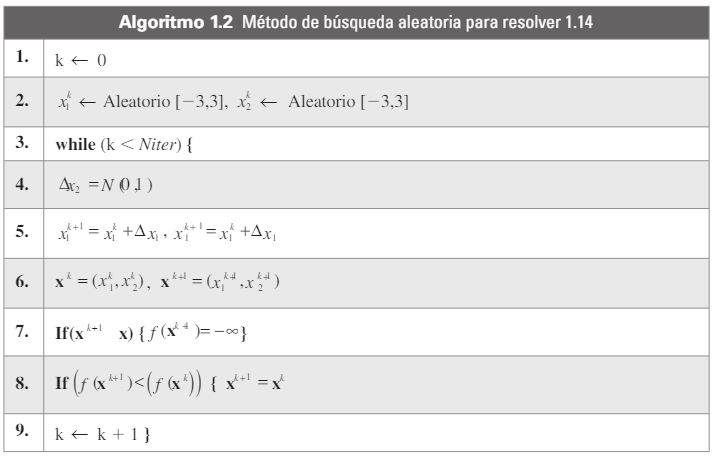
\includegraphics[width=15cm]{imgs/busqueda_aleatoria.JPG}
    \caption{Algoritmo de B\'usqueda Aleatoria}
    \label{fig:my_label}
\end{figure}

\subsubsection{Temple Simulado}
El temple simulado o en ingl\'es 'Simulated annealing' es una t\'ecnica de optimizaci\'on que emula el proceso de templado en materiales met\'alicos. La idea del templado es enfriar el material controladamente de tal manera que las estructuras cristalinas puedan orientarse y evitar los defectos en las estructuras met\'alicas. \\ El uso del templado como inspiraci\'on para la formulaci\'on de algoritmos de optimizaci\'on fue por primera vez propuesto por Kirkpatrick, Gelatt y Vecchi en 1983. Desde entonces se han sugerido varios estudios y aplicaciones para analizar los alcances del m\'etodo.A diferencia de algoritmos basados en gradiente, el m\'etodo del temple simulado presenta una gran habilidad para evitar quedar atrapados en los m\'inimos locales.\\En el templado simulado, el valor de la función objetivo que se intenta optimizar es análogo a la energía de un sistema termodinámico. En altas temperaturas el algoritmo permite la exploración de puntos muy distantes entre sí en el espacio de búsqueda, además de que la probabilidad de aceptación de soluciones que no mejoran su estado anterior es muy grande. Po el contrario, a bajas temperaturas, el algoritmo permite \'unicamente la generaci\'on de puntos muy cercanos entre s\'i, adem\'as de que la probabildiad de aceptaci\'on se reduce, por lo que ahora s\'olo las nuevas soluciones que mejoren su estado anterior, ser\'an consideradas.\\El \textit{algoritmo de temple simulado} matiene urante su funcionamiento una sola soluci\'on candidato $(x^k)$. Dicha soluci\'on es modificada en cada iteraci\'on utilizando un procedimiento similar al de m\'etodo de b\'usqueda aleatoria, donde cada punto es modificado mediante la generaci\'on de un vector aleatorio $\Delta x$. Sin embargo, este algoritmo no solo acepta los cambios que mejoren su funci\'on objetivo, sino que incorpora un mecanismo probabil\'istico, que le permite aceptar incluso soluciones que le empeoren. Esto con el fin de salir de los m\'inimos locales.

Bajo estas circunstancias, una nueva soluci\'on ser\'a aceptada $x^{k+1}$ considerando dos diferentes alternativas
\begin{itemize}
    \item Si su calidad es superior a la de su antecesor $x^k$. Esto es si $f(x^{k+1})>f(x^k)$
    \item Bajo una probabilidad de aceptaci\'on $p_a = e^{\frac{\Delta f}{T}}$, donde $T$ representa la temperatura que controla el proceso de templado, mientras que $f$ es la diferencia de energ\'ia entre el puntos $\Delta f= f(x^{k+1})-f(x^k)$
\end{itemize}
A continuaci\'on mostramos el algoritmo de temple simulado.
\begin{figure}[h!]
    \centering
    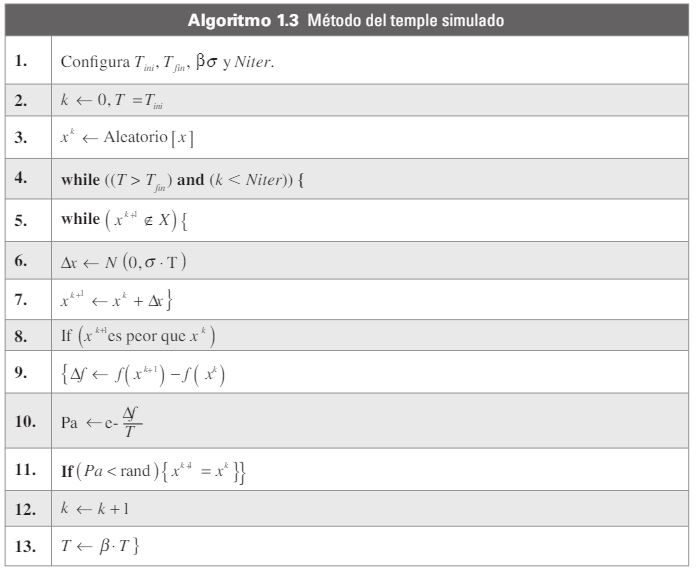
\includegraphics[width=15cm]{imgs/templado_simulado.JPG}
    \caption{Caption}
    \label{fig:my_label}
\end{figure}
\subsubsection{Gen\'eticos}
Un algoritmo genético es un método de búsqueda que imita la
teoría de la evolución biológica de Darwin para la resolución de
problemas. Para ello, se parte de una población inicial de la cual
se seleccionan los individuos más capacitados para luego
reproducirlos y mutarlos para finalmente obtener la siguiente
generación de individuos que estarán más adaptados que la
anterior generación.
\subsubsection{Implementación}
Una premisa es conseguir que el tamaño de la población sea lo
suficientemente grande para garantizar la diversidad de
soluciones.
Los pasos básicos de un algoritmo genético son:
\begin{itemize}
\item Evaluar la puntuación de cada uno de los cromosomas
generados.
\item Permitir la reproducción de los cromosomas siendo los
más aptos los que tengan más probabilidad de
reproducirse.
\item Con cierta probabilidad de mutación, mutar un gen del
nuevo individuo generado.
\item Organizar la nueva población
\end{itemize}
Se puede fijar un número máximo de iteraciones
antes de finalizar el algoritmo genético o detenerlo cuando no se
produzcan más cambios en la población.

Parametros de los algoritmos geneticos.
\begin{itemize}
    \item Tamaño de la población.
    \item Probabilidad de cruce.
    \item Probabilidad de mutación.
\end{itemize}

Al igual que en otros algoritmos metaheurísticos, los AG presentan algunas ventajas respecto a los métodos clásicos de optimización; por ejemplo, pueden trabajar con poca o ninguna información acerca de la función objetivo, y por ser poblacionales tienen mayores probabilidades de escapar de óp-timos locales, en comparación con los métodos determinísticos. Sin embargo, entre sus desventajas está el hecho de que no garantizan una convergencia al óptimo real, y en muchos casos son más tardados que las técnicas deterministas

\subsubsubsection{Un ejemplo}
Veamos como aplicar un algoritmo genetico para minimizar la siguiente función . la cual es dificil desde el punto de vista computacional, pues contiene bastantes optimos locales 

\begin{align*}
    f(x_1,x_2)=a+exp(1)-a*exp(-b\sqrt{\frac{1}{d}(x_1^2+x_2^2)})-exp(\frac{1}{d}(\cos{c_1x_1}+\cos{c_2x_2}))\\
    x_1,x_2 \in [-15,30]
\end{align*}


\begin{verbatim}
    function [temp, ind] = FUNCION(x, d, N) y=[];% 
    Ackley
    for j=1:N       
       a = 20; b = 0.2; c = 2*pi;   
       s1 = 0; s2 = 0;    
       for i=1:d;        
          s1 = s1+x(j,i)^2;       
          s2 = s2+cos(c*x(j,i));   
    end
    y(j,1) = -a*exp(-b*sqrt(1/d*s1))-exp(1/d*s2)+a+exp(1);
    end
    [temp,ind]=sort(y);
\end{verbatim}

Básicamente un AG es un programa que genera una población inicial aleatoria de padres, y durante cada generación selecciona pares de padres, considerando su valor de $f(x_i,)$, para realizar intercambios de material genético, o cruza, y generar pares de hijos; tales hijos serán mutados con una cierta probabilidad, y nalmente competirán por sobrevivir a la siguiente generación con los padres, proceso que se conoce como elitismo. Aunque dicho comportamiento produce la convergencia del algoritmo, también es cierto que provoca que la población sea ‘arrastrada’ por el mejor individuo de la población, lo que conduce en ocasiones un estancamiento de la población

La desventaja de esto es que podria llegarse encontrar un optimo local en ves de uno global

\subsubsection{Estrategias Evolutivas}

Las EE son algoritmos inspirados en la evolución y al igual que otros basados en tal metáfora, sus individuos realizarán una “evolución”, o mejora, con respecto a alguna función objetivo y mediante operadores que imitan dicho proceso.

Podriamos por ejemplo considerar minimizar $f$ tal que:
\begin{align*}
   f(x_1,x_2)=-sen(x1)sen^{2m}(\frac{x_1^2}{\pi})+sen(x_2)sen^{2m}(\frac{2x_2^2}{\pi}
   x_1,x_2 \in [0,\pi]
   m=10
\end{align*}

Para ello podemos implementar el siguiente codigo

\begin{verbatim}
    function [f, i1] = FUNCION(x, d, mu) 
    y=[];
    for i1=1:mu   
    m = 10;   s = 0;   
    for i2 = 1:d       
    s = s + sin(x(i1,i2))*(sin(i2*x(i1,i2)^2/pi))^(2*m);   
    end   
    y(i1,1) = -s; 
    end
    [f, i1]=sort(y);
\end{verbatim}
Esta función en particular tambien presenta minimos locales por lo que es dificil estudiarla al menos con las estrategias que conocemos hasta el momento
Esencialmente, los operadores que se utilizan en las EE son muy parecidos a los de un AG, cuando menos nominalmente; sin embargo, la diferencia más notoria es que en las EE el operador de mutación no es un solo valor, sino una matriz de valores de mutación. Esta es una de sus características más interesantes, e incluso se considera como la más importante.
La principal diferencia en la inicialización en las EE con respecto a otros algoritmos evolutivos radica en que se crean las matrices de covarianza y rotaciones $(\sigma,\alpha)$

Se muestra a continuación las principales estrategias a seguir para generar un algoritmo evolutivo.
\begin{figure}[h!]
    \centering
    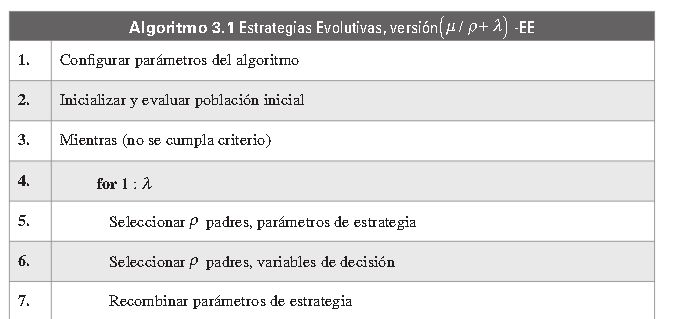
\includegraphics[width=10cm]{imgs/Captura de pantalla 2021-01-19 184554.png}
    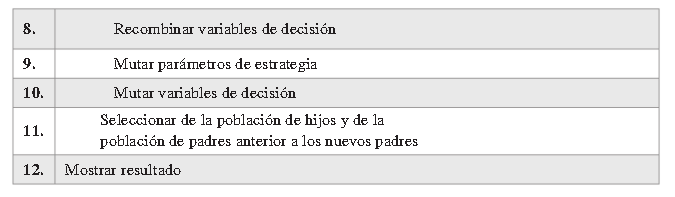
\includegraphics[width=10cm]{imgs/Captura de pantalla 2021-01-19 184634.png}
    \caption{Muestra de un algoritmo evolutivo}
    \label{fig:my_label}
\end{figure}




\subsubsection{Evoluci\'on Diferencial}
El algoritmo de Optimizaci\'on Evoluci\'on Diferencial (Differential Evolution, por sus siglas en ingl\'es), es un algoritmo poblacional de b\'usqueda directa y simple, el cual es capaz de optimizar hasta alcanzar el \'optimo global en funciones multimodales, no diferenciales y no lineales. Fue propuesto por \textit{Kenneth Price y Rainer Storn} en $1995$. Desde entonces, el algoritmo DE ha probado sus capacidades en concursos Internacionales de la IEEE en Optimizaci\'on Evolutiva, asi como con grandes aplicaciones en el mundo real.

El DE se basa en perturbar a los miembros de la poblaci\'on generada con diferencias escaladas de distintos miembros de una misma poblaci\'on. Lo hacen caracter\'istico de los dem\'as algoritmos evolutivos dado que esta inspirado en un f\'enomeno biol\'ogico, social, f\'isico o qu\'imico. El algoritmo DE fue dise\~nado para que se cumpliera con (i) capacidad de lidiar con funcio-nes objetivo no diferenciables, no lineales y multimodales, (ii) fácil implementación, (iii) pocos parámetros de ajuste, (iv) propiedades de convergencia consistentes en pruebas consecutivas in-dependientes y (v) capacidad de paralelizarse para lidiar con funciones de alto costo computa-cional. A continuaci\'on se presenta el algoritmo o un diagrama de flujo g\'enerico de las operaciones llevadas acabo por el algoritmo evoluci\'on diferencial.
\begin{figure}[h!]
    \centering
    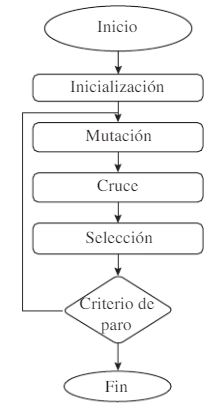
\includegraphics[width=5cm]{imgs/Evolucion diferencial.JPG}
    \caption{Caption}
    \label{fig:my_label}
\end{figure}
De acuerdo cone studios reportados recientemente, el algoritmo DE ha mostrado un mejor desempe\~no que muchos algoritmos evolutivos en t\'erminos de convergencia, velocidad y robustez sobre distintas funciones de prueba.

\subsubsection{B\'usqueda Arm\'onica}
En este algoritmo se representa a una armonía como en vector $n$-dimensional de números reales.
\begin{itemize}
    \item Un conjunto inicial de vectores de armonía son generados aleatoriamente y almacenados dentro de la memoría de armonías (HM).
    \item Una nueva armonía candidada es calculada a partir de los elementos contenidos en la HM, para esto existe un parámetro conocido como consideración de memoria.
    \item Se actualiza la memoria de armonías, por medio de la comparación de la nueva armonía candidata y el peor de los vectores de armonía. 
\end{itemize}
\begin{figure}[H]
    \centering
    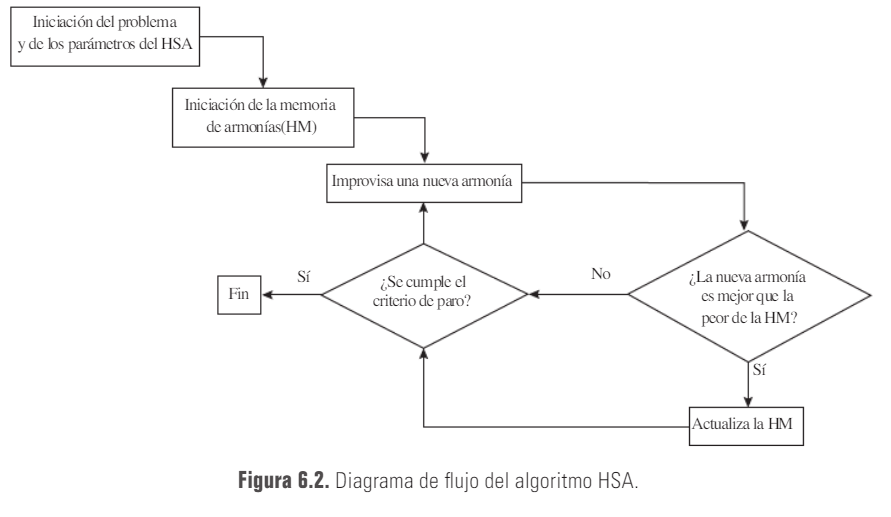
\includegraphics[scale=0.6]{imgs/hsa_diagrama.png}
\end{figure}
Un popularidad del algoritmo HSA se debe a un conjunto de características que lo distinguen del resto de los algoritmos metaheurísticos. Algunas de éstas son: \\ 
1. Para generar nuevas soluciones se consideran todas las soluciones existentes, no sólo dos de ellas como los padres en los algoritmos genéticos. \\ 
2. Se considera de forma independiente cada variable de decisión en un vector de soluciones. \\
3. Los valores de las variables de decisión son continuos, por lo que no se pierde precisión.

\subsubsection{Sistemas Inmunológicos Artificiales}
Para definir lo que es un sistema inmune artificial recurriremos a una de
las definiciones más completa propuesta por Leandro Nunes de Castro y
Jonathan Timmis. \\Los sistemas inmunes artificiales son sistemas adaptativos, inspirados por la teoría inmunológica, funciones, principios y modelos inmunológicos observados, los cuales son aplicados a la
solución de problemas.\\
Aunque la cantidad de modelos y aplicaciones del sistema inmune va en
ascenso, no existe un esquema general de cuáles son los elementos esenciales
que un sistema inmune artificial debe poseer. \\
Nunes De Castro y Timmis sugieren en su libro utilizar un esquema
general de sistemas computacionales con inspiración biológica, tal como los
algoritmos evolutivos o las redes neuronales. Este esquema consta de tres
partes principales que deben denirse, y que a continuación se muestran:

\begin{itemize}
  \item  Representación de los componentes del sistema.
  \item Un conjunto de mecanismos para evaluar las interacciones de los individuos con el ambiente y entre ellos.
  \item Un proceso de adaptación que gobierne las dinámicas del sistema, es
decir, el algoritmo en sí.
\end{itemize}

 Representación de los componentes del sistema.\\
 Un conjunto de mecanismos para evaluar las interacciones de los individuos con el ambiente y entre ellos.\\
 Un proceso de adaptación que gobierne las dinámicas del sistema, es
decir, el algoritmo en sí.\\

A diferencia de otras técnicas bio-inspiradas (por ejemplo los algoritmos
genéticos), el sistema inmune artificial no tiene un algoritmo general único.












\subsubsection{Optimizaci\'on basada en electromagnetismo}
El algoritmo EMO es un método basado en población propuesto por Birbil y Fang  para resolver modelos de optimización continuos usando variables acotadas. Es decir,  problemas de optimización.
El algoritmo EMO replica el problema de las cargas, donde cada carga representa una solución a un campo dado, lo cual representa que cada cantidad de carga es una parte de la solución y refleja su cálidad. Este algoritmo, permite encontrar solución a problemas de minimización del tipo $f(X) X \epsilon [l,u]$ a través de los siguientes cuatro pasos.

\begin{itemize}
    \item Inicialización: un conjunto de m partículas son tomadas aleatoriamente considerando un espacio $R$ definido por el límite superior u y el límite inferior l
    \item Búsqueda local: se realiza la búsqueda de un valor mínimo en la vecindad de un punto $X_p$, donde $ p \epsilon [m1,m2]$ y m es el número total de individuos de la población.
    \item Cálculo del vector de fuerza total: con base en el valor de la función objetivo se calculan las cargas y fuerzas para cada elemento de población de partículas.
    \itemMovimiento: cada partícula de población es desplazada de acuerdo a la fuerza total calculada con base en el valor de la función objetivo.
\end{itemize}
\begin{verbatim}
%Inicializacion, Algoritmo EMO Standar
%Prueba con función de Rosenbrock
function [x.fx] = inicializa (m,n,u,l)
%Se genera las partículas de forma aleatoria en el espacio de búsqueda
for i = 1:n
%Se obtiene el número aleatorio
lambda= rand(l,m);
	x(i,:) = l(i) + lambda * (u(i) -l(i));
end
%Se evalúa cada partícula en la función objetivo (Rosenbrock)
for j =1:m
	fx(j) = rosen(x(:,j));
end             
\end{verbatim}

El código anterior es una implementación del algoritmo EMO para la función de Rosenbrock.
\subsubsection{Colonia Artificial en Abejas, Hormigas}
El problema de optimización de colonia, es una tecnica probabilística para resolver problemas computacionales que pueden ser reducidos a encontrar un camino bueno en una gráfica. \\ 

La forma más fácil de entender como el algoritmo de optimización por colonia de hormigas funciona, es a través de un ejemplo. Consideremos el problema del agente viajero, consiste en, dado un conjunto de ciudades y la distancia entre estas, encontrar la ruta más corta que visite a todas y regrese al lugar de partida. \\

Las hormigas construyen la solución de la siguiente manera. Cada hormiga selecciona una ciudad aleatoria. Después, en cada paso se mueve a un nuevo vértice queno haya sido visitado de forma probabilística, esta decisión esta basada en información como la feromona. Cada vez que una hormiga finaliza su recorrido, la feromona de cada arista es actualizado de acuerdo a la calidad de la solución resultante.

\section{Estudiar, evaluar y argumentar la elección de algún algoritmo evolutivo.}
\subsection{Estudio.}
El algoritmo genético como ya mencionamos en la sección anterior, es un algoritmo que restringe una búsqueda con los siguientes pasos.
\begin{itemize}
    \item Generar población inicial.
    \item Seleccionar de esta población individuos más capacitidados.
    \item Reproducir y mutar estos individuos.
    \item Obtiene una nueva generación de individuos mejor adaptados
    
\end{itemize}
El proceso se repite hasta llegar a una solución aceptable.
El algoritmo genético podemos notar que se basa de un sistema de selección natural, en el cual tras cada iteración solo los individuos más aptos sobreviven, y que por tanto serán base para las generaciones posteriores.
Esta capacidad les permite resolver muchos problemas que no son de un capo en específico. Solo debemos definir un problema y una función de evaluzación de los individuos para poder resolver cualquier tipo de problema. Al traterse de una técnica heurística el tiempo de ejecución puede volverse un obstáculo si el espacio de búsqueda de soluciones es muy amplio, además de que si el factor de mutación no es elegido con cuidado, podríamos hacer un algirtmo que no convergiese a el óptimo búscado. Por eso es necesario garantizar la diversidad de los individuos al realizar la técnica, y también es esta complicación por la cual es natural aplicar paralelización, precisamente en la sub sección siguiente discutiremos esto con más profundidad, para dar la justificación a la elección de un algoritmo genético.

\begin{center}
    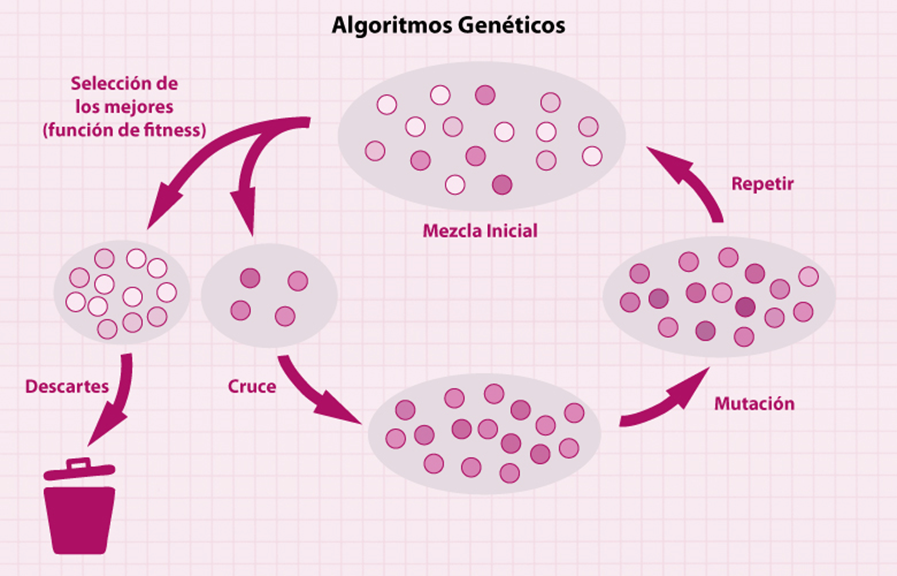
\includegraphics[scale = 0.5]{ALGORITMOGENETICO2.png}
\end{center}


\subsection{Evaluación}

\subssubsection{Justificación}
Decidimos elegir el algoritmo genético dado que la labor de selección de los individuos, es una tarea que se puede paralelizar y que además no afecta la solución final del algoritmo. La selección debe ser realizada de manera global si queremos que el algoritmo produzca el mismo resultado que el secuencial original. Otro punto del algoritmo donde se puede realizar la paralelización de la población, podemos en lugar de generar una población muy grande, grupos pequeños de poblaciones que se comuniquen entre ellas, esté punto es el que de acuerdo a la bibliografía más apremia realizar una paralelización contra el secuencial ya que incluso puede ser algo favorable, comenzar con sub poblaciones para la búsqueda, incluso este proceso de paralelización se conoce como generar nichos.
\begin{center}
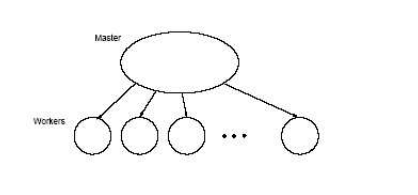
\includegraphics[scale=0.8]{imgs/AGP.png}    
\end{center}
Esta es una representación esquemática de un algoritmo genético paralelizado, con la aplicación del proceso paralelo en la evaluación de los individuos, ya que suele ser también la que toma más tiempo. 

    El intercambio de información entre los nodos 
realiza los siguientes pasos
\begin{itemize}
    \item Nodo maestro envia subconjunto de individuos a cada nodo. 
    \item Cada nodo retorna el valor de evaluación al nodo maestro.
    
\end{itemize}
De forma tradicional, el nodo maestro espera a recibir los valores de adecuación de todos los individuos para hacer la siguiente generación, pero también podemos hacer que los nodos más lentos no se comuniquen con el nodo maestro, aunque aquí perderíamos información del comportamiento original.

\begin{center}
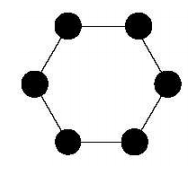
\includegraphics[scale =1]{imgs/arqui2.png}    
\end{center}

Una segunda forma de generar paralelización, es generar una arquitectura de muchas poblaciones, este es el caso en donde cada sub población es repartida hacía un diferente procesador y es evaluada por separado. Se encontró que en está arquitectura, las poblaciones por separado convergen más rápido hacía valores óptimos, aunque en contraste, estos valores no son tan buenos como los del proceso secuencial.






\section{Problema de aplicación elegido en el punto anterior}
El problema de aplicación es colorear una gráfica de $n$ vértices con $3$ colores, esto es, dado $G(E,V)$ debemos asignare un color a cada vértice de tal forma que no haya dos vértices adyacentes que sean del mismo color.
\begin{figure}[H]
    \centering
    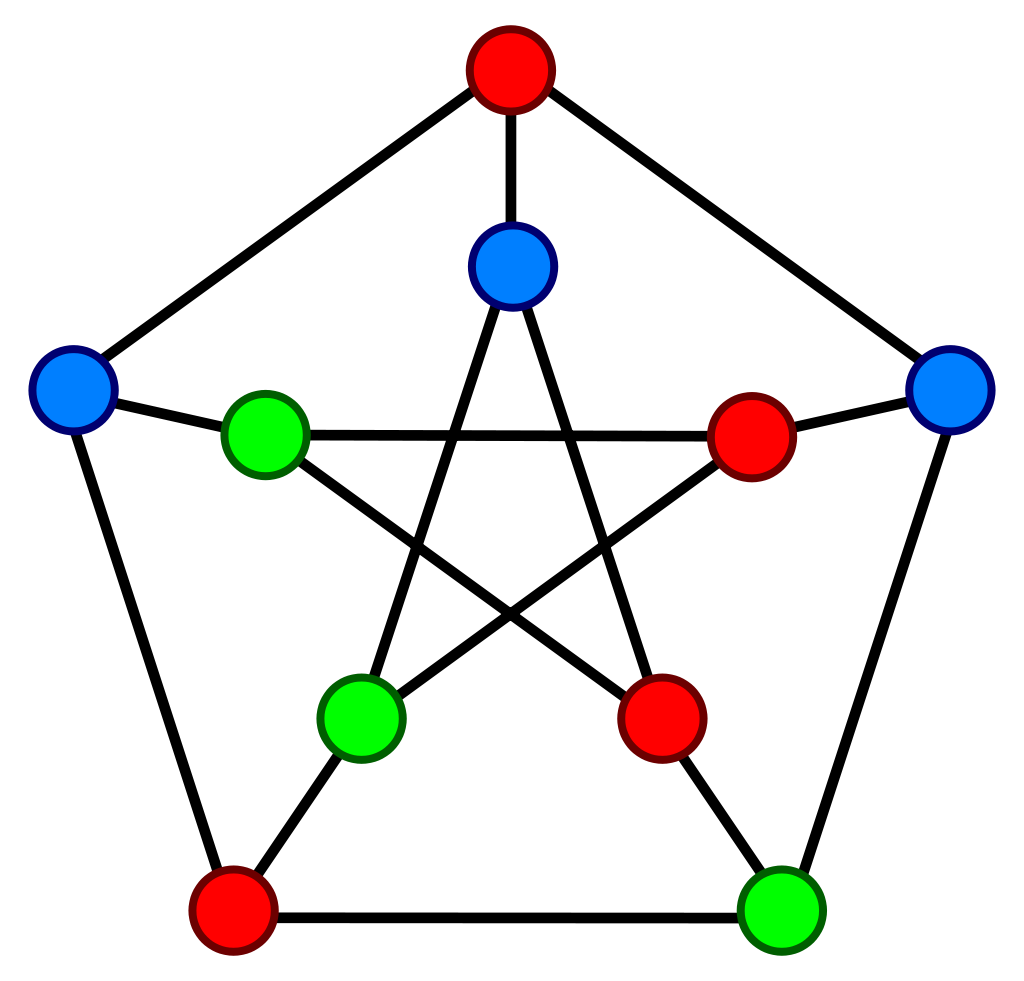
\includegraphics[scale=0.2]{imgs/graph_3color.png}
\end{figure}
En este caso se tienen las siguientes definiciones:
\begin{itemize}
    \item Person: Una coloración arbitraria de la gráfica, esta se puede ver como un array que nos indica el color 
    de cada vertice $[1,0,2,1,...,0]$.
    \item Fitness: Número de aristas que conectan a dos vértices del diferente color.
    \item Crossover: Dadas 2 gráficas (padres) elegimos un número aleatorio entre $0$ y $n$ y creamos una nueva gráfica que tenga los primeros $k$ colores iguales a los de la primera y el resto igual a los de la segunda.
\end{itemize}
El procedimiento es el siguiente:
\begin{enumerate}
    \item Generar población aleatoria (primer generación).
    \item Obtener fitness.
    \item Obtener a los individuos con mayor fitness.
    \item Hacer crossover para obtener nueva generación.
    \item Repetir paso 2
\end{enumerate}
El modelo tiene los siguientes hyper-parámetros:
\begin{itemize}
    \item population\_size: Número de personas en la población.
    \item n\_nodes: Número de nodos aleatorios de la gráfica
    \item n\_generations: Número de generaciones que se usarán para evolucionar a la población.
    \item percentage\_keep: Porcentaje de la población con mejor fitness que se copia de a la siguiente población. 
\end{itemize}

\section{Programa - Simulación}
Para la simulación se utilizara python y la libreria networkx junto con matplotlib asi como multiprocessing lo que nos permitira implementar nuestro algoritmo de manera paralela.
\begin{pythoncode}
ds
\end{pythoncode}

\section{Conclusiones}

\begin{thebibliography}{}
\bibitem{}\textsc{Coley, D. A}  Introduction to Genetic Algorithms for Scientists and Engineers. (First ed.).

\bibitem{}\textsc{Goldberg, D } Genetic Algorithms in Search, Optimization, and Machine Learning. Addison-Wesley Professional.
\end{thebibliography}

\bibitem[]{}En la referencia "Optimización. Algoritmos programdos con MATLAB", Cuevas et al., Alfaomega, México, 2016, podrán encontrar los siguientes algoritmos evolutivos: 

\end{document}
